\documentclass[12pt, twoside, openany]{report}
% pacote usado para que os capítulos, figuras, etc., fiquem em português brasileiro.
\usepackage[brazil]{babel}
% pacote usado para permitir escrita de palavras com acentos diretamente no texto latex.
\usepackage[utf8]{inputenc}
% pacote usado para melhorar a hifenização
\usepackage[T1]{fontenc}
\usepackage{ae} % fontes quase europeias :) (almost european)
\usepackage{verbatim}
\usepackage{enumitem} %alterar label da numeração
\usepackage{subfig} %mais de uma figura por imagem
\usepackage{float} %forçar posição de figura
\linespread{1.5} % espaçamento entre linhas
\usepackage{geometry} % permite o uso do pacote para configuração da geometria do documento de forma facilitada
\geometry{a4paper, left = 2cm, right = 2cm, top = 2cm, bottom = 2cm}
\usepackage[dvipdfm]{hyperref} % hiper referência p/ pdf
\hypersetup{bookmarksnumbered = true,           % bookmarks numerados
            colorlinks = true,                  % links coloridos
            linkcolor = blue,                   % cor dos links
            citecolor = blue,                   % cor das citações
            urlcolor = blue,                    % \href{. . .}{. . .} URL externa
            filecolor = green,                  % \href{. . .}{. . .} arquivo local
            }
\usepackage{graphicx}

\begin{document}

%%%%%%%%%%%%%%%%%%%%%%%%%%%%%%%%%%%%%%%%%%%%%%%%%%%%%%%%%%%%
%%%%%                CAPA 					
%%%%%%%%%%%%%%%%%%%%%%%%%%%%%%%%%%%%%%%%%%%%%%%%%%%%%%%%%%%%
\thispagestyle{empty}

\noindent 
\rule{\textwidth}{1ex}\\

\begin{center}
\Large \textbf{Instituto Federal do Norte de Minas Gerais \\ IFNMG -- Campus Montes Claros \\}
\textbf{Bacharelado em Ciência da Computação}

\vspace{1cm}
\Huge {\textcolor{blue}{\textbf{Análise do Perfil Empreendedor}}}

\vfill

\Large \textbf{David Jansen, Eike Stálei, Iarah Almeida, \\ Marianna Leandra e Roberta Rasoviti}
\vfill

\Large \textbf{Última atualização: \today}
\end{center}

 \noindent 
 \rule{\textwidth}{1ex}\\[1ex]

%%%%%%%%%%%%%%%%%%%%%%%%%%%%%%%%%%%%%%%%%%%%%%%%%%%%%%%
% estilo de numeração das páginas do sumário...
\newpage \pagenumbering{roman} 
\tableofcontents

%%%%%%%%%%%%%%%%%%%%%%%%%%%%%%%%%%%%%%%%%%%%%%%%%%%%%%%
% estilo de numeração das páginas de todo o texto e configuração para exibição do cabeçalho e rodapé...
\newpage \pagenumbering{arabic} \pagestyle{headings} 

%%%%%%%%%%%%%%%%%%%%%%%%%%%%%%%%%%%%%%%%%%%%%%%%%%%%%%%
%       Iniciar os capítulos...
%%%%%%%%%%%%%%%%%%%%%%%%%%%%%%%%%%%%%%%%%%%%%%%%%%%%%%%
% Cada capítulo será escrito em arquivos .tex separados 
% e serão inseridos via comando \include
\begin{abstract}
\addcontentsline{toc}{chapter}{Resumo}
-----
\end{abstract}
\chapter{Introdução}\label{capitulo1}

"O empreendedor é uma pessoa que enxerga uma \textbf{oportunidade} aliada a um \textbf{sonho} ou uma ideia, tem \textbf{coragem} para colocá-la em prática e criar um \textbf{diferencial} relacionado ao novo negócio, um projeto social ou mesmo uma inovação dentro do ambiente de trabalho" (Santos e Souza2013 Falta achar referência). Quando posta em prática, a oportunidade se torna um produto (tangível ou intangível) que pode vir a trazer importantes benefícios à sociedade, como foram os grandes inventos: avião e computador.

 O termo \textit{empreendedor} data de um período remoto. Os primeiros empreendedores surgiram no Século XIII, período do explorador Marco Polo, atuando de forma ativa no comércio através da rota com o oriente. No Brasil, a existência de empreendedores se intensificou nos anos 90, e consolidou-se em 2000. Isso se deve a variações econômicas que incentivam aos de "mente inovadora” a criarem novas alternativas e soluções para o mercado. Atualmente existem empresas especializas em desenvolver esse espírito do empreendedor de forma técnica, tornando os empreendedores também bons administradores, por exemplo, o Sebrae e a Empretec. Eventos patrocinados ou incentivados por tais empresas costumam cultivar a criação de startups que são empresas com foco em funcionamento imediato e com forte potencial de crescimento. Muitas empresas hoje consolidadas e com alto capital surgiram como startups. Entre essas empresas estão a Google, Facebook, Uber e Airbnb.
    
As Startups são comumente associadas à tecnologia e fundadas por membros jovens. O IFNMG - \textit{Campus} Montes Claros oferece cursos técnicos de informática e química, duas áreas com amplo potencial para inovação. Diante desse fato, o presente trabalho pretende analisar o perfil empreendedor dos alunos de ambos os cursos citados, afim de compreender a visão dos alunos sobre o empreendedorismo e possivelmente desenvolver eventos, atividades, palestras e dinâmicas que possam os instigar e orientar para serem empreendedores de sucesso.
\chapter{Metodologia}\label{capitulo2}

Para realizar nossa análise do perfil empreendedor, utilizamos de um questionário composto somente de perguntas objetivas (Consulte o apêndice \ref{Questionario}) divididas em dois grupos: perguntas para analisar do perfil social do aluno \textbf{(Grupo S)} e perguntas para analisar habilidades e conhecimentos relacionados ao perfil empreendedor \textbf{(Grupo E)}. Este questionário foi mapeado em um modelo do Google Forms e então aplicado, por meio da divulgação do link de acesso, às turmas de 1º, 2º e 3º ano dos cursos de Técnico em Informática e Técnico em Química do IFNMG - Campus Montes Claros. O formulário ficou aberto durante duas semanas e foram recolhidas 58 respostas.

\section{Dados da Pesquisa}
Inicialmente, a própria ferramenta do Google nos fornece algumas informações sobre o perfil social do aluno utilizando da distribuição das respostas por curso, por ano, por gênero, por moradia e por possuir ou não renda pessoal (\ref{fig:quest1-5}).

Ainda utilizando o Google Forms, recolhemos as informações gráficas sobre as distribuições das respostas pertencentes ao grupo E: características do empreendedor (\ref{fig:caract}) e crenças sobre o empreendedorismo (\ref{fig:mv1-2}, \ref{fig:mv3-4} e \ref{fig:mv5}).

\begin{figure}[!htb]
    \centering
    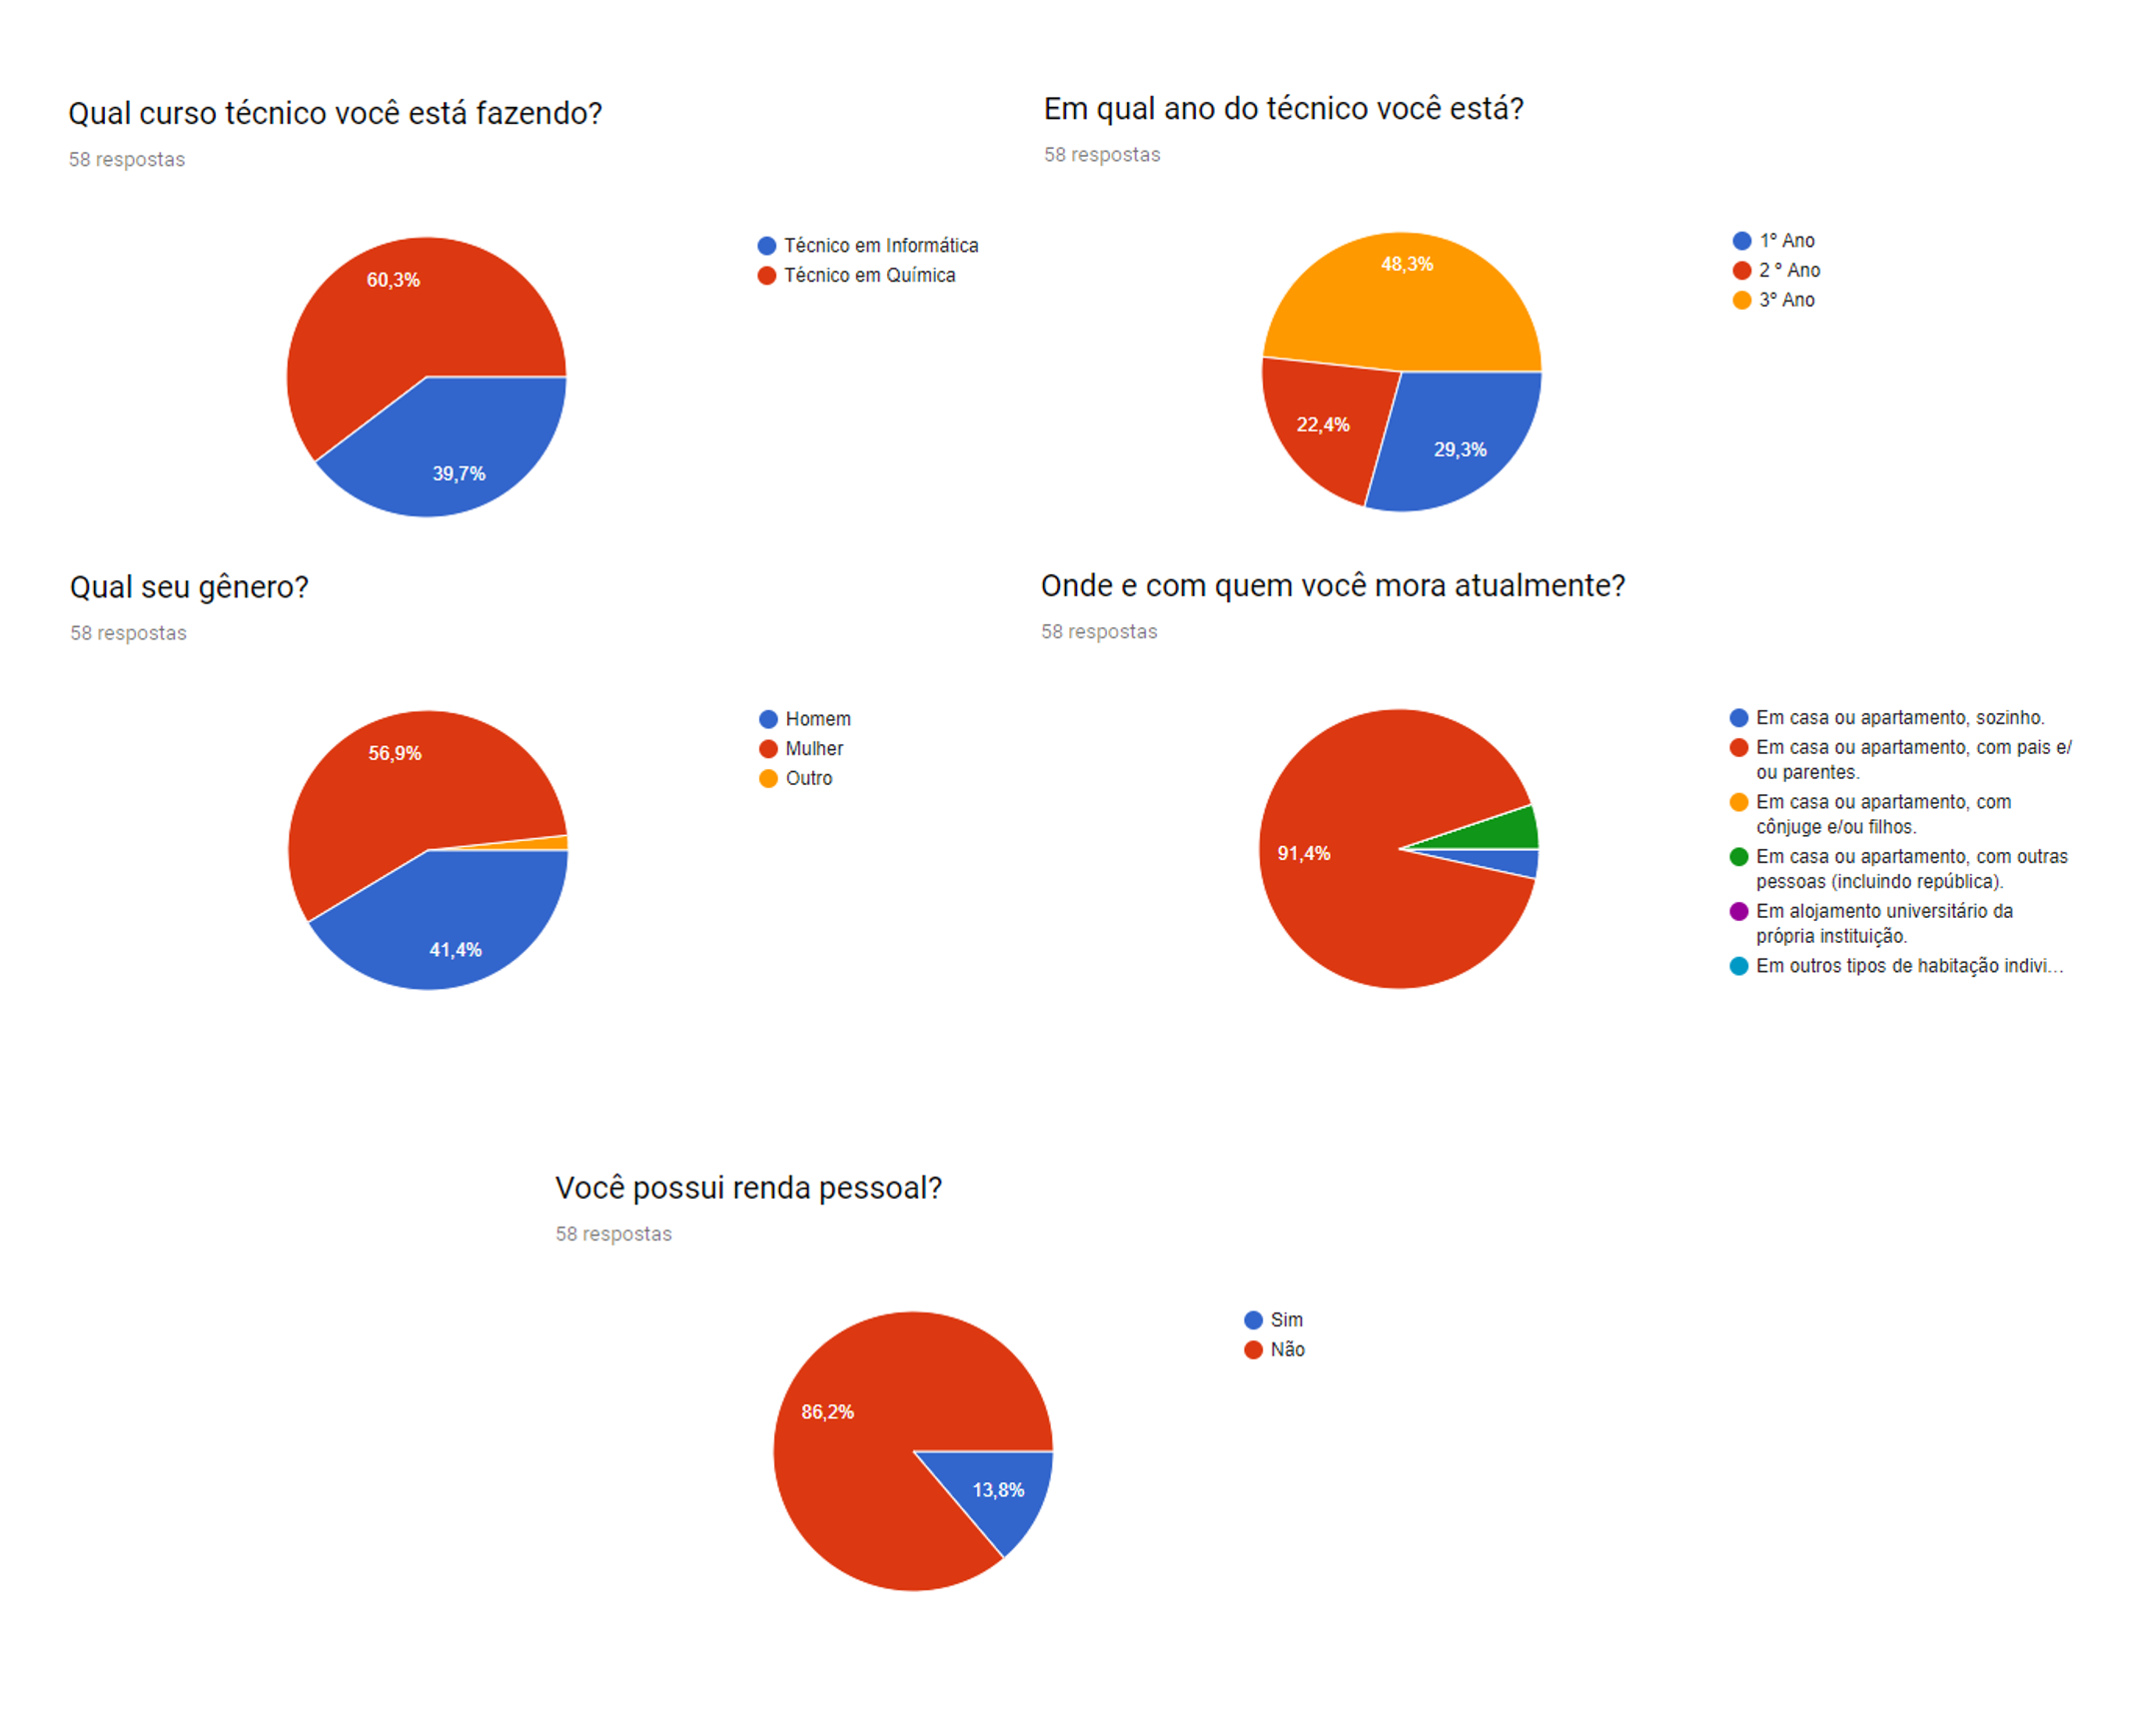
\includegraphics[width=1.0\textwidth]{img/quest1-5.png}
    \caption{Perguntas n$^{\underline{\circ}}$ 1 a 5}
    \label{fig:quest1-5}
\end{figure}

\begin{figure}[!htb]
    \centering
    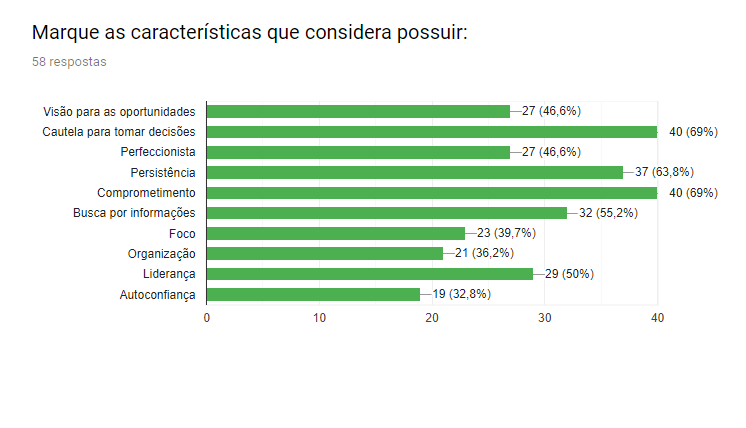
\includegraphics[width=0.9\textwidth]{img/habilidades.PNG}
    \caption{Características que os alunos acreditam possuir.}
    \label{fig:caract}
\end{figure}

\begin{figure}[!htb]
    \centering
    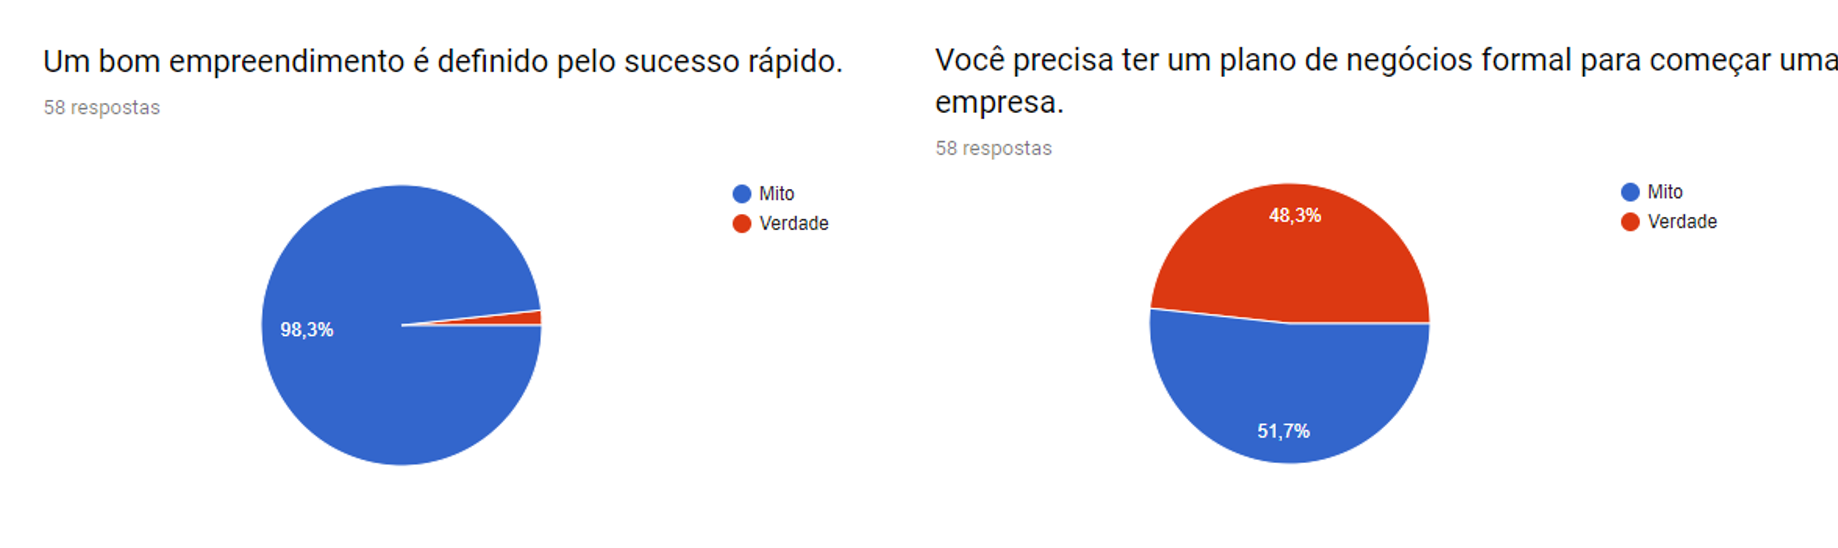
\includegraphics[width=1.0\textwidth]{img/mv1-2.png}
    \caption{Mitos e Verdades (a : Mito) e (b : Mito).}
    \label{fig:mv1-2}
\end{figure}

\begin{figure}[!htb]
    \centering
    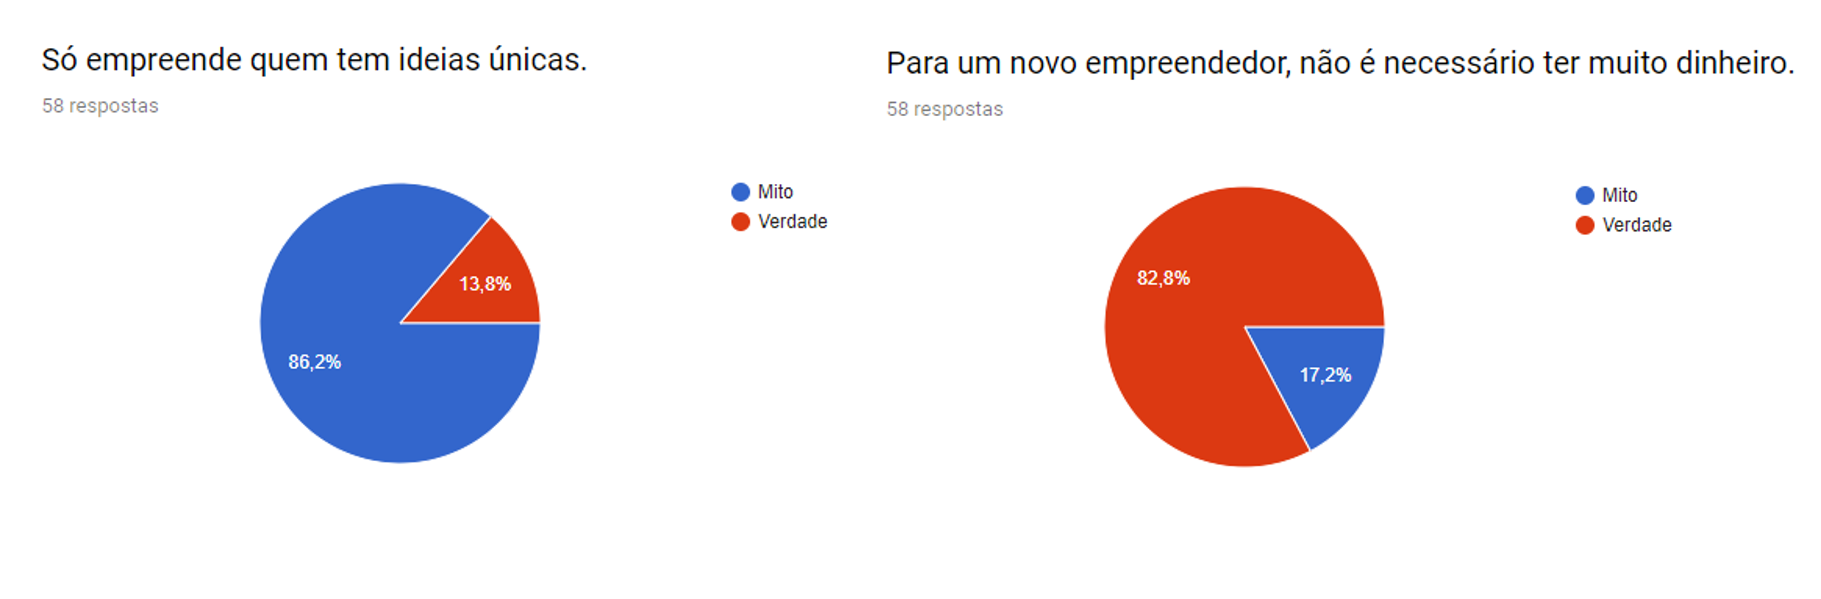
\includegraphics[width=1.0\textwidth]{img/mv3-4.png}
    \caption{ Mitos e Verdades (c : Mito) e (d : Verdade).}
    \label{fig:mv3-4}
\end{figure}

\begin{figure}[!htb]
    \centering
    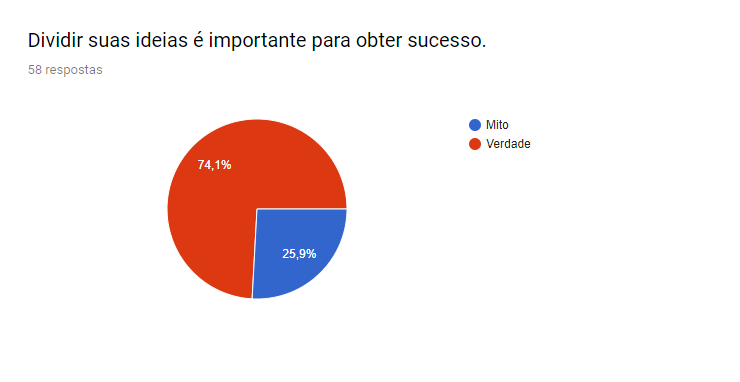
\includegraphics[width=0.7\textwidth]{img/mv5.PNG}
    \caption{Mitos e Verdades (e : Verdade)}
    \label{fig:mv5}
\end{figure}



\appendix
\chapter{Questionário}\label{Questionario}

\begin{enumerate}[noitemsep]
    \item Qual curso técnico você está fazendo?
    \begin{enumerate}[noitemsep]
        \item Técnico em informática
        \item Técnico em química
    \end{enumerate}
    \item Em qual ano do técnico você está?
    \begin{enumerate}[noitemsep]
        \item 1º
        \item 2º
        \item 3º
    \end{enumerate}
    \item Qual seu gênero?
    \begin{enumerate}[noitemsep]
        \item Homem
        \item Mulher
        \item Outro
    \end{enumerate}
    \item Onde e com quem você mora atualmente?
    \begin{enumerate}[noitemsep]
        \item Em casa ou apartamento, sozinho.
        \item Em casa ou apartamento, com pais e/ou parentes.
        \item Em casa ou apartamento, com cônjuge e/ou filhos.
        \item Em casa ou apartamento, com outras pessoas (incluindo república).
        \item Em alojamento universitário da própria instituição.
        \item Em outros tipos de habitação individual ou coletiva (hotel, hospedaria, pensão ou outro)
    \end{enumerate}
    \item Você possui renda pessoal?
    \begin{enumerate}[noitemsep]
        \item Sim
        \item Não
    \end{enumerate}
    \item Marque as características que considera possuir:
    \begin{enumerate}[noitemsep]
        \item Visão para as oportunidades
        \item Cautela para tomar decisões
        \item Perfeccionismo
        \item Persistência
        \item Comprometimento
        \item Buscar por informações
        \item Foco
        \item Organização
        \item Liderança
        \item Autoconfiança
    \end{enumerate}
    \item Mitos e Verdades.
        \begin{enumerate}[noitemsep]
            \item Um bom empreendimento é definido pelo sucesso rápido.
            \begin{enumerate}[noitemsep]
                \item Verdade
                \item Mito
            \end{enumerate}
            \item Você precisa ter um plano de negócios formal para começar uma empresa.
            \begin{enumerate}[noitemsep]
                \item Verdade
                \item Mito
            \end{enumerate}
            \item Só empreende quem tem ideias únicas.
            \begin{enumerate}[noitemsep]
                \item Verdade
                \item Mito
            \end{enumerate}
            \item Para um novo empreendedor, não é necessário ter muito dinheiro.
            \begin{enumerate}[noitemsep]
                \item Verdade
                \item Mito
            \end{enumerate}
            \item Dividir suas ideias é importante para obter sucesso.
            \begin{enumerate}[noitemsep]
                \item Verdade
                \item Mito
            \end{enumerate}
            \item O empreendedor corre riscos sem planejamento.
            \begin{enumerate}[noitemsep]
                \item Verdade
                \item Mito
            \end{enumerate}
        \end{enumerate}
\end{enumerate}


\bibliography{bibliografia}
\bibliographystyle{plain}

%\appendix
%\include{Apendice1}

\end{document}
